\documentclass{article}
\usepackage{amsmath}
\usepackage{graphicx}
\usepackage[utf8]{inputenc}
\usepackage[T1, T2A]{fontenc}
\usepackage[english,russian]{babel}

\newcommand{\p}{\partial}

\title{Нелинейный осциллятор\\ в поле вращающейся волны}
\author{Anikin Evgeny}

\begin{document}
\maketitle
Гамильтониан нелинейного осциллятора во внешнем поле имеет вид
\begin{equation}
   \hat{H} = \omega_0 a^\dagger a + \frac{\beta}{2} a^\dagger a^\dagger a a + 
                E^*e^{i\Omega t} a + Ee^{-i\Omega t} a^\dagger 
\end{equation}
Преобразованием $\Psi = e^{i\Omega t a^\dagger a} \widetilde{\Psi}$ уравнение Шрёдингера
приводится к виду
\begin{equation}
    i\partial_t \widetilde{\Psi} = \hat{H}_{\mathrm{eff}}\widetilde{\Psi},
\end{equation}
где 
\begin{equation}
    \hat{H}_{\mathrm{eff}} = (\omega_0 - \Omega) a^\dagger a + 
                        \frac{\beta}{2} a^\dagger a^\dagger a a + 
                E^* a + Ea^\dagger 
\end{equation}
Этот гамильтониан, в принципе, можно диагонализовать и тем самым найти полный набор решений
исходного уравнения Шрёдингера. Однако в такой постановке непонятно, как понимать
бистабильность. Найденные решения соответствуют как стационарным, так и нестационарным решениям
классического уравнения для консервативного осциллятора. Поэтому в задачу необходимо ввести
диссипацию. Для этого введём взаимодействие с баней осцилляторов:
\begin{equation}
    \begin{gathered}
        \hat{H}_{\mathrm{full}} = \hat{H} + \hat{H}_\mathrm{bath} + \hat{H}_\mathrm{int}, \\
        \hat{H}_\mathrm{bath} = \sum \omega_k b_k^\dagger b_k \\
        \hat{H}_\mathrm{int} = \sum \gamma_k a^\dagger b_k + \mathrm{h. c.}
    \end{gathered}
\end{equation}
Тут тоже можно сделать такое преобразование волновой функции, чтобы гамильтониан стал
независящим от времени: $\Psi = \exp{i\Omega t(a^\dagger a + 
\sum b_k^\dagger b_k)}\widetilde{\Psi}$. 
Тогда эффективный гамильтониан примет вид
\begin{multline}
    \hat{H}_\mathrm{eff} = (\omega_0 - \Omega) a^\dagger a + 
                        \frac{\beta}{2} a^\dagger a^\dagger a a + 
                E^* a + Ea^\dagger + \\
                + \sum (\omega_k - \Omega) b_k^\dagger b_k + 
                \sum \gamma_k a^\dagger b_k + \mathrm{h. c.}
\end{multline}
Этот гамильтониан описывает нелинейный осциллятор, взаимодействующий с баней. Существенно, 
что в этой бане присутствуют осцилляторы как с положительной, так и с отрицательной энергией.
Благодаря этому возможно такое равновесие осциллятора, что он только испускает "фотоны" бани,
а не поглощает. 

Рассмотрим испускание фотонов осциллятором на полуклассическом языке. Предположим, мы нашли
собственные состояния $\hat{H_\mathrm{eff}}$. Тогда вероятность перехода в единицу времени
 между уровнями
$n$ и $m$ ---
\begin{equation}
    \begin{gathered}
        \frac{dP(m \leftarrow n)}{dt} \propto | \gamma_k \langle m | \hat{a} | n \rangle|^2,\\
        \omega_k - \Omega = E_n - E_m
    \end{gathered}
\end{equation}
Тогда можно написать кинетическое уравнение на вероятности находиться на $m$--ом уровне:
\begin{equation}
    \frac{dP_m}{dt} = \sum_n \frac{dP(m \leftarrow n)}{dt} P_n - \frac{dP(n \leftarrow m)}{dt} P_m
\end{equation}
Если найти стационарное распределение вероятностей, то при определённых значениях параметров 
у него будет два пика. Это и будет соответствовать бистабильности.

Матричные элементы $ \langle m | \hat{a} | n \rangle$ легко найти численно. Тогда будут
определены и вероятности перехода, если известны $\gamma_k$. Последние можно задать
каким--нибудь разумным способом, например, $\gamma(E) \propto \theta(E)$ или
$\gamma(E) \propto E$. После этого можно будет найти стационарное распределение вероятностей.

\begin{figure}[h]
    \centering
    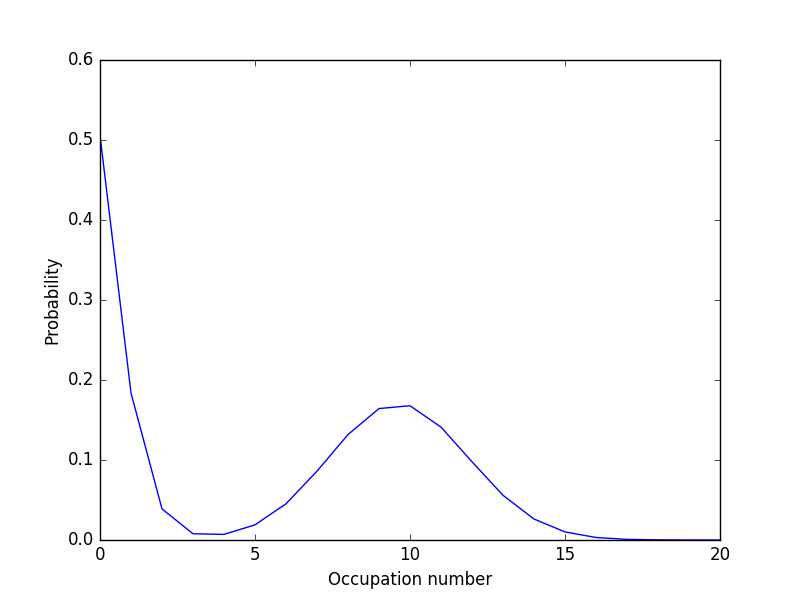
\includegraphics[width=0.7\textwidth]{bistability.png}
    \caption{Вероятности чисел заполнения нелинейного осциллятора при следующих параметрах:
             $\omega_0 = 1$,
             $\Omega=1.025$,
             $\beta=0.003$,
             $E=0.0138$}
\end{figure}
\end{document}
